\documentclass{article}

\usepackage[margin=1.0in]{geometry}
\usepackage{graphicx}
\usepackage{amsmath}
\usepackage{float}
\usepackage{enumitem}

\title{CSC 535 HW8}
\date{12/01/2018}
\author{Simon Swenson}

\begin{document}

\pagenumbering{gobble}
\maketitle
\pagenumbering{arabic}

\large Introduction

\small I completed both question one and two. Generally, the implementation was 
straightforward with few bugs. One caveat that I missed was expanding the log 
terms in the log likelihood to cancel the exponent, so I was originally getting 
weird points that would have $-\infty$ log likelihood due to floating point 
rounding, but after fixing that, the program seemed to work without a hitch.

\section{Q1}

The main part of this project was implementing the EM algorithm for GMMs. Thus, 
there were really four main tasks to the project:

\begin{itemize}
    \item calculating responsibilities, given cluster means, covariance 
        matrices, and priors
    \item calculating priors, given responsibilities
    \item calculating means, given responsibilities
    \item calculating covariance matrices, given means
\end{itemize}

The first task is the "expectation" step, and the last three tasks 
constitute the "maximization" step. These operations are encapsulated in the Gmm 
class in gmm.py. In addition to the main algorithm, it is also important to be 
able to get statistical information over the course of the algorithm. In my 
code, this is done using an observer pattern, an object of class 
"DefaultGmmObserver." This class has callbacks which the Gmm object will call 
at certain points during its execution. This allows me to generalize the stopping 
condition as well as calculate the log likelihoods for each iteration of the 
algorithm.

Finally, the program contains a function for calculating the probability 
density for a given point, mean, and covariance matrix and the "main" code at 
the bottom, which also saves the various plots.

One quirk about this algorithm is that it will only find local maxima of the 
log likelihood function. This is due to its iterative nature. Just like 
gradient descent, it will always settle at an extremum, but that extremum may be 
different. In addition, this depends quite a lot on the data set, itself. I 
noticed that, for some data sets, like the first one, the clusters always 
seemed to settle at the same spots with $k = 3$. (See figure 1).

\begin{figure}[!ht]
	\centering
	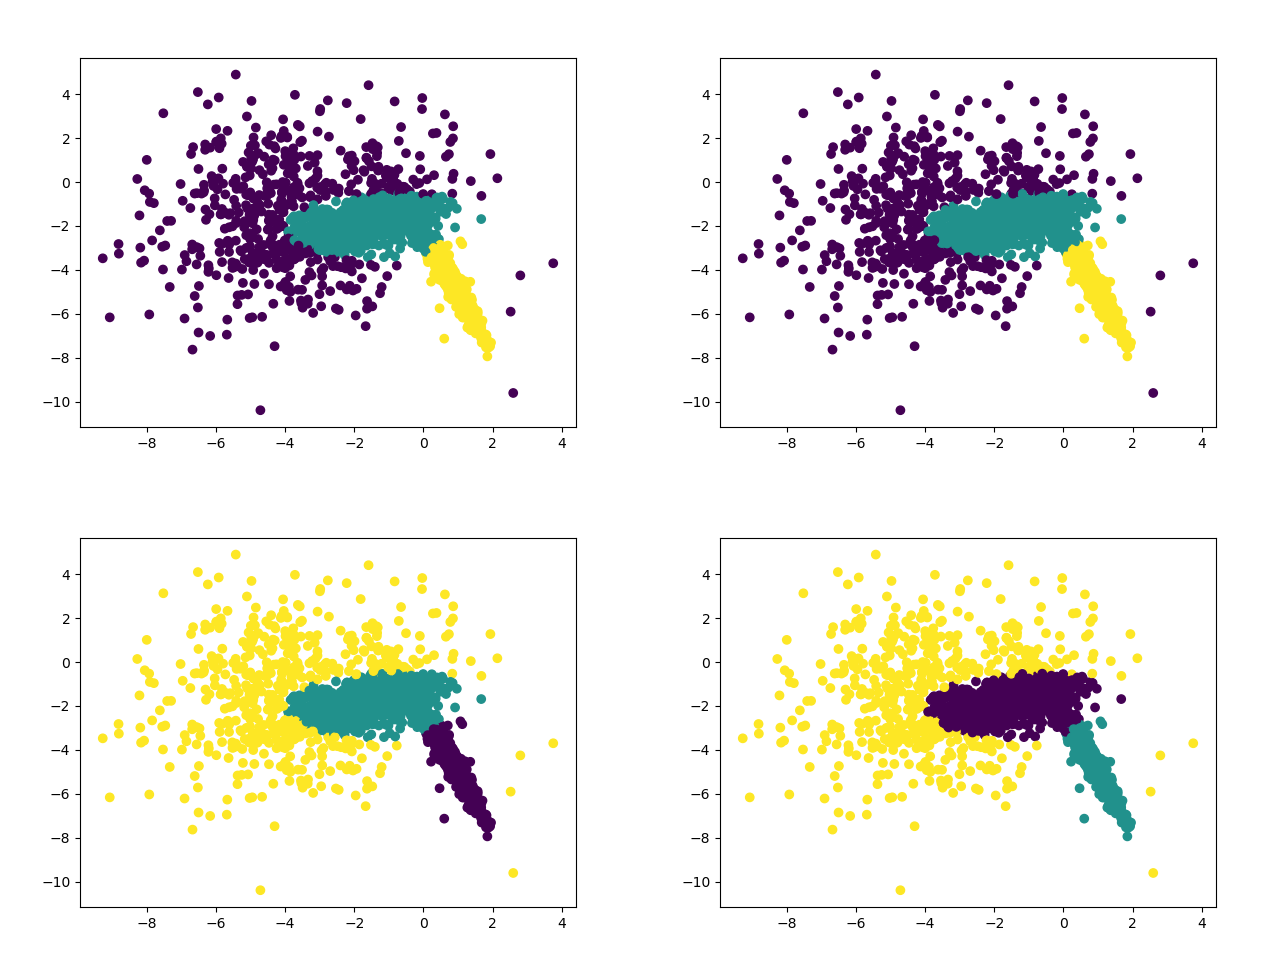
\includegraphics[width=120mm]{figs/gmm_ds0_k3_orthog_plt_4trials.png}
	\caption{The result of the GMM clustering of four random initializations for 
        the first data set with $k = 3$. They are roughly the same.}
\end{figure}

~\\
~\\
~\\
~\\
~\\
~\\
~\\
~\\
~\\
~\\
~\\
~\\
~\\
~\\
~\\
~\\
~\\

This similarity is also visible in the clustering of the third data set. (See figure 2.)

\begin{figure}[!ht]
	\centering
	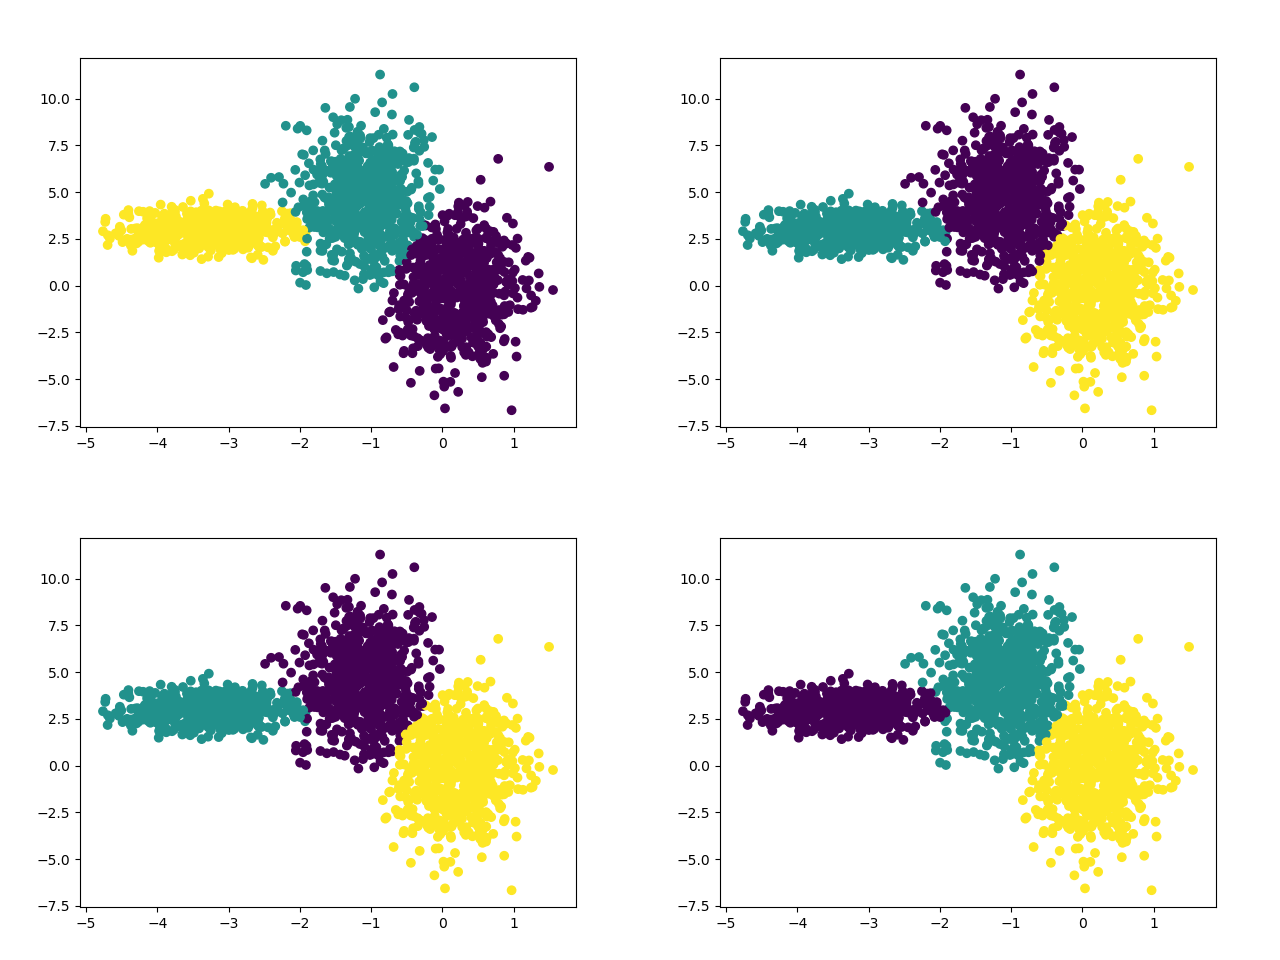
\includegraphics[width=120mm]{figs/gmm_ds2_k3_orthog_plt_4trials.png}
	\caption{The result of the GMM clustering of four random initializations for 
        the third data set with $k = 3$. They are roughly the same.}
\end{figure}

Perhaps these trials are not the best trials to show the effects of random 
initialization. One configuration that did have a substantial difference 
based on initialization, however, was the second data set with $k = 5$. (See figure 3.)

\begin{figure}[!ht]
	\centering
	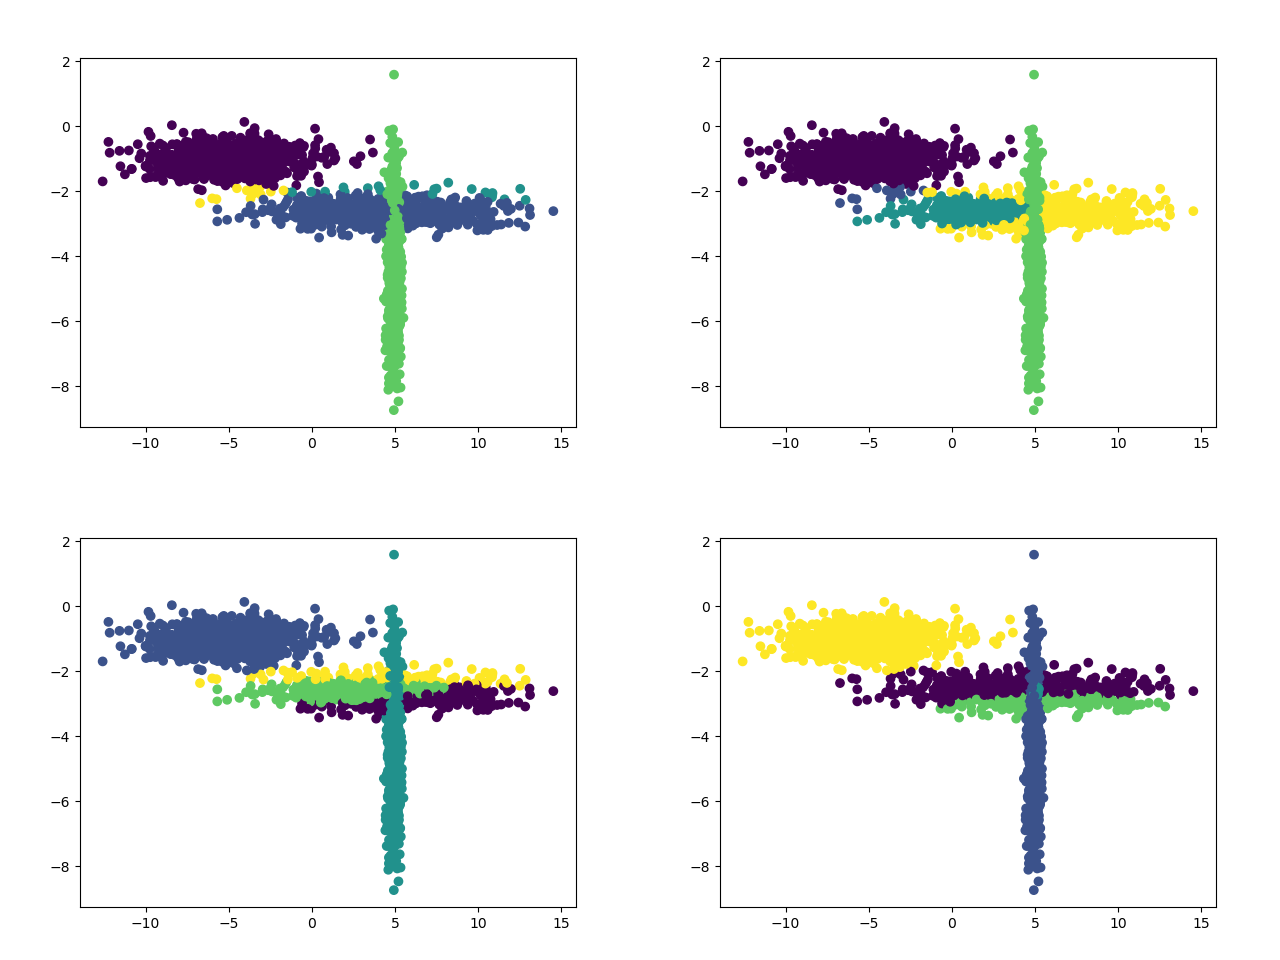
\includegraphics[width=120mm]{figs/gmm_ds1_k5_orthog_plt_4trials.png}
	\caption{The result of the GMM clustering of four random initializations for 
        the second data set with $k = 5$. This shows a substantial difference, 
        depending on initialization.}
\end{figure}

Since we have found a counter-example, it is clear that clustering is, indeed, 
a function of initialization.

~\\

In addition to examining the output clustering of the algorithm, an important 
metric to consider is the objective function, itself, the log likelihood. In the 
experiments, the main trend that I noticed was that, initially, the log 
likelihood (of both training and test data) does not exhibit much of a change. 
My intuition for this is that the random initialization really throws the 
algorithm into the "deep end of the pool," so to speak. Once the algorithm has 
previous values that make sense, but are not ideal, it can improve on them, but 
starting at a completely random spot makes these first few iterations slower. 
The algorithm has to find its bearings.

After this latent period, the log 
likelihood exhibits a period of rapid change for several iterations. However, 
the training log likelihood and the test log likelihood go in opposite 
directions. As we proved in class, the EM algorithm will \textit{always} 
increase the training log likelihood. However, test log likelihood exhibits a 
different pattern: it rapidly decreases at this point in the algorithm. This did 
not immediately make sense to me. If test data is roughly in the same spot as 
training data, then it should have a similar log liklihood, I thought.
Initially, I thought this might be a sign of the dreaded "overfitting," but I 
don't really think that overfitting is much of a concern in clustering, since 
there are no labels to which to overfit. Instead, I would say that this decrease in 
log likelihood is simply a reflection of the fact that we are not training with 
that data, so our GMM is less likely to \textit{explain} it. It's a slighly 
different explanation than "overfitting."

Finally, the log likelihood tapers off. This is essentially where the algorithm has 
reached the extremum that it was heading to. This would be a good place to stop, 
so maybe exploring different values for delta would be fruitful to stop at the 
\textit{start} of this era instead of spending quite a few iterations inside of it. (See figure 4.)

\begin{figure}[!ht]
	\centering
	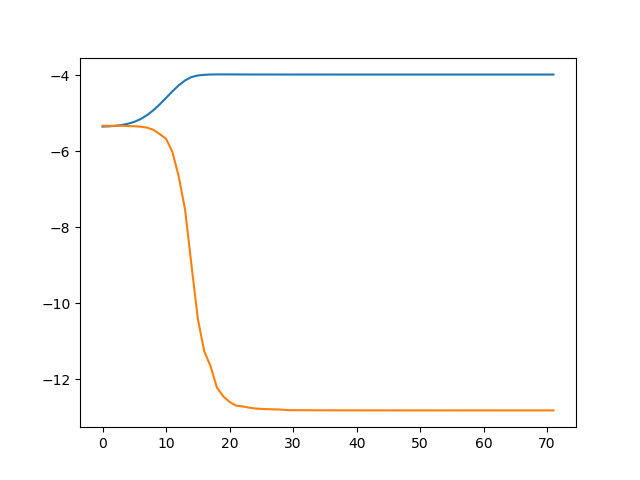
\includegraphics[width=120mm]{figs/gmm_ds0_k3_orthog_ll_trial4.png}
	\caption{A typical example of the log likelihood curves. Here, we used dataset one with $k = 3$. 
        Training log likelihood is blue, test log likelihood is orange.}
\end{figure}

~\\
~\\
~\\
~\\
~\\
~\\
~\\
~\\

Here are typical results for the six datasets, with both $k=3$ and $k=5$, 
showing both the final clustering and the log likelihood charts. (See figures 5-10.) One interesting 
note is that, with a $k$ the same as the $k$ used to generate the data set, the 
GMM is \textit{much} more likely to converge to the same clustering. Another 
important note is that, because Gaussians are, essentially, ovals, GMM has 
trouble with squarish datasets. This can be seen in the fifth data set. Finally, 
since we used diagonal covariance matrices, the ovals could not take on any 
interesting angles. This can be seen in the first data 
set, as two of the clusters should be angled but are not. (Compare to the 
results from the non-diagonal covariance matrices below.)

\begin{figure}[!ht]
	\centering
	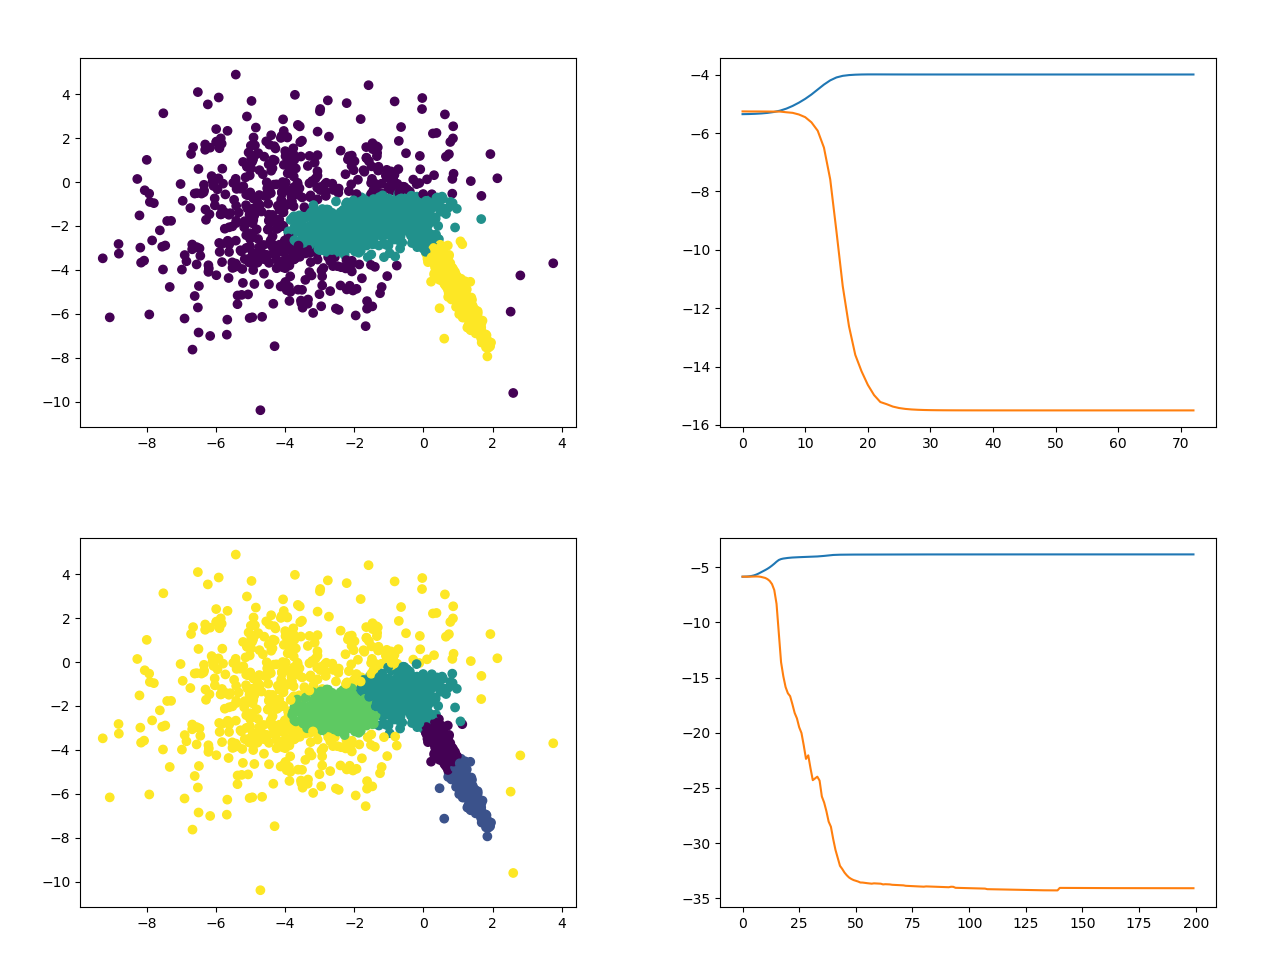
\includegraphics[width=120mm]{figs/gmm_ds0_orthog_plt_ll.png}
	\caption{Results for the first data set. TL: clustering with $k = 3$, TR: log likelihood with $k = 3$, BL: clustering with $k = 5$, BR: log likelihood with $k = 5$.}
\end{figure}

\begin{figure}[!ht]
	\centering
	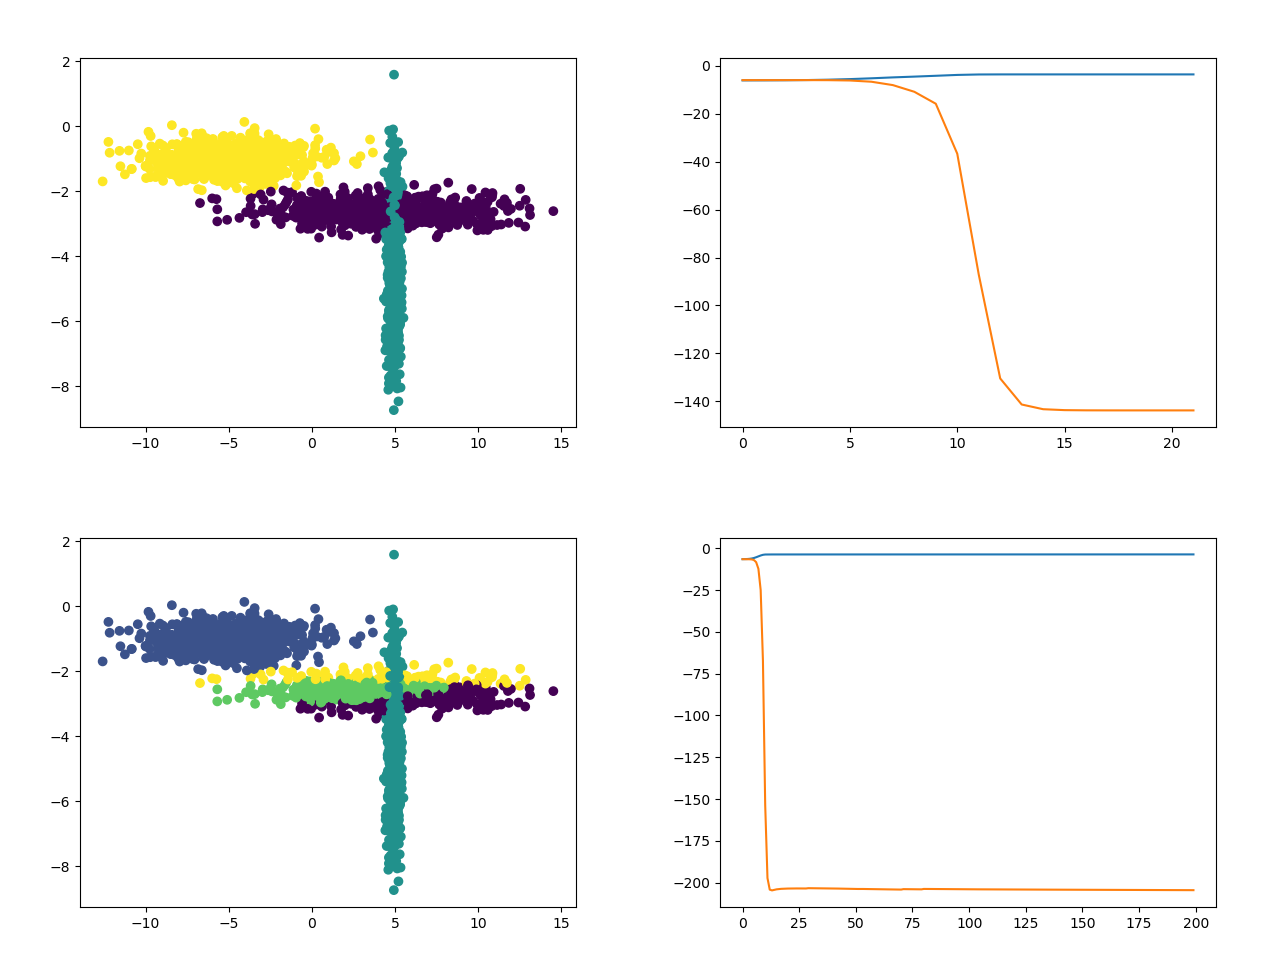
\includegraphics[width=120mm]{figs/gmm_ds1_orthog_plt_ll.png}
	\caption{Results for the second data set. TL: clustering with $k = 3$, TR: log likelihood with $k = 3$, BL: clustering with $k = 5$, BR: log likelihood with $k = 5$.}
\end{figure}

\begin{figure}[!ht]
	\centering
	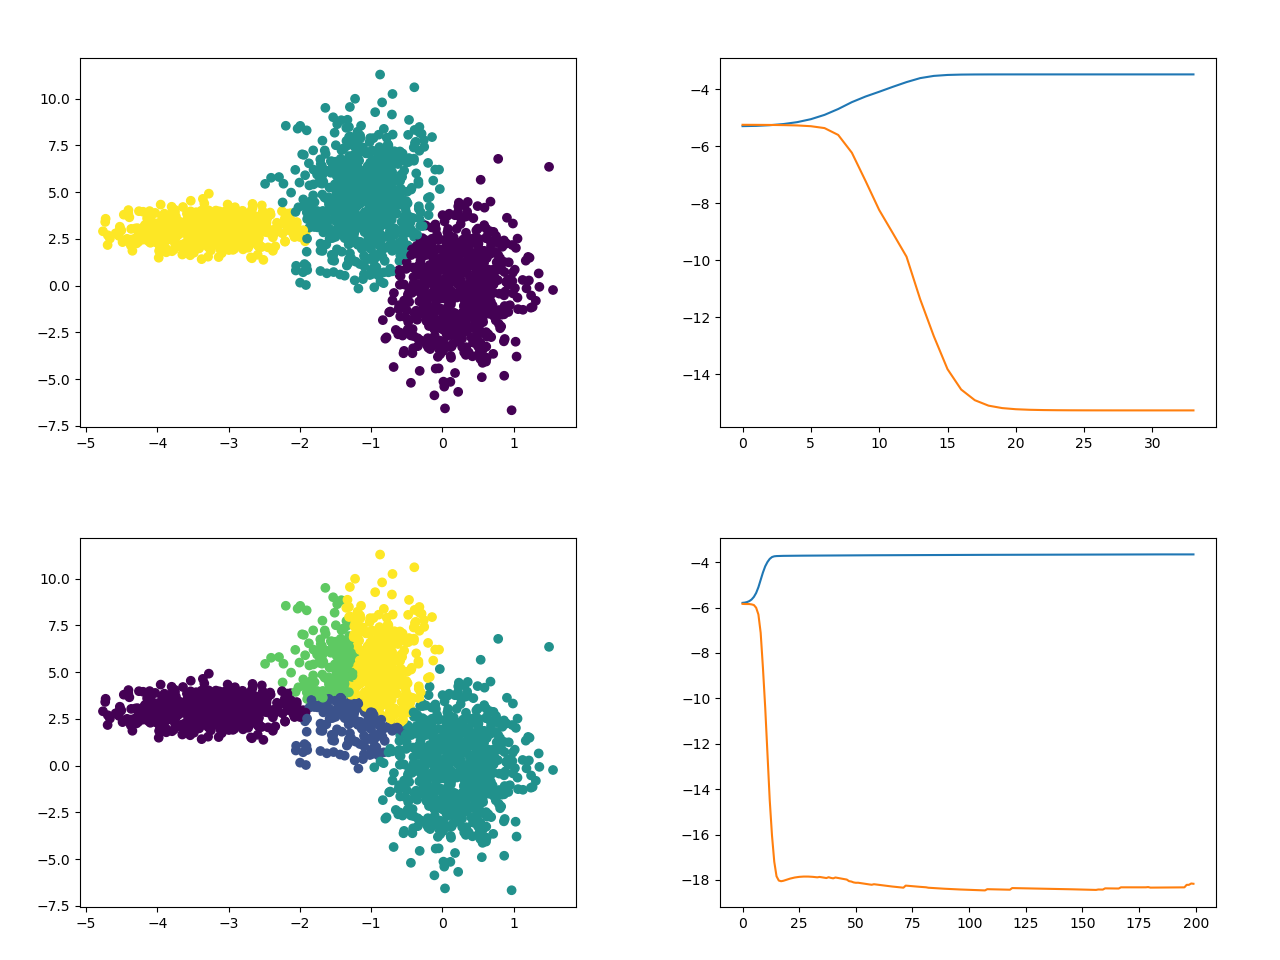
\includegraphics[width=120mm]{figs/gmm_ds2_orthog_plt_ll.png}
	\caption{Results for the third data set. TL: clustering with $k = 3$, TR: log likelihood with $k = 3$, BL: clustering with $k = 5$, BR: log likelihood with $k = 5$.}
\end{figure}

\begin{figure}[!ht]
	\centering
	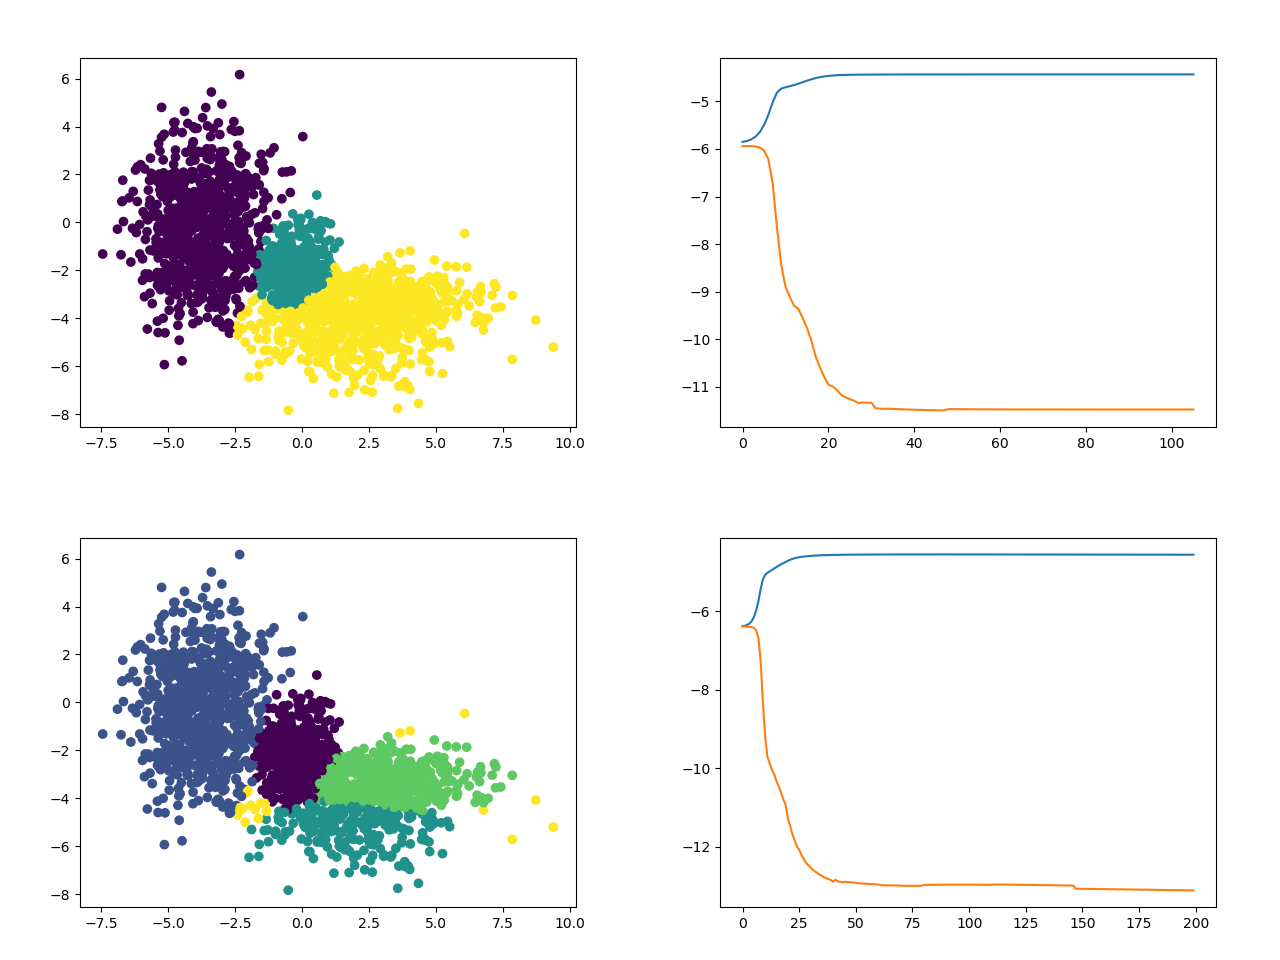
\includegraphics[width=120mm]{figs/gmm_ds3_orthog_plt_ll.png}
	\caption{Results for the fourth data set. TL: clustering with $k = 3$, TR: log likelihood with $k = 3$, BL: clustering with $k = 5$, BR: log likelihood with $k = 5$.}
\end{figure}

\begin{figure}[!ht]
	\centering
	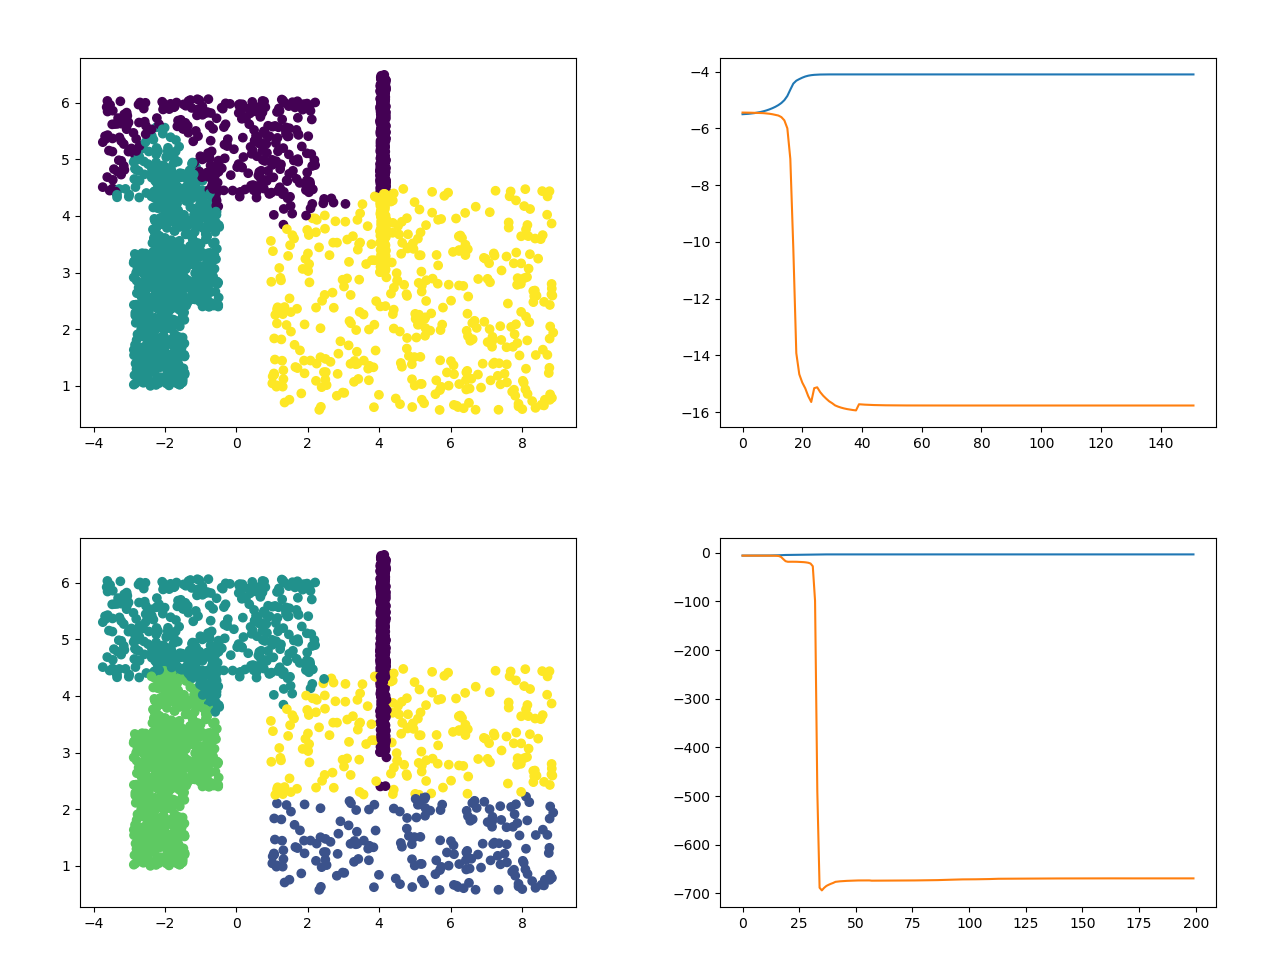
\includegraphics[width=120mm]{figs/gmm_ds4_orthog_plt_ll.png}
	\caption{Results for the fifth data set. TL: clustering with $k = 3$, TR: log likelihood with $k = 3$, BL: clustering with $k = 5$, BR: log likelihood with $k = 5$.}
\end{figure}

\begin{figure}[!ht]
	\centering
	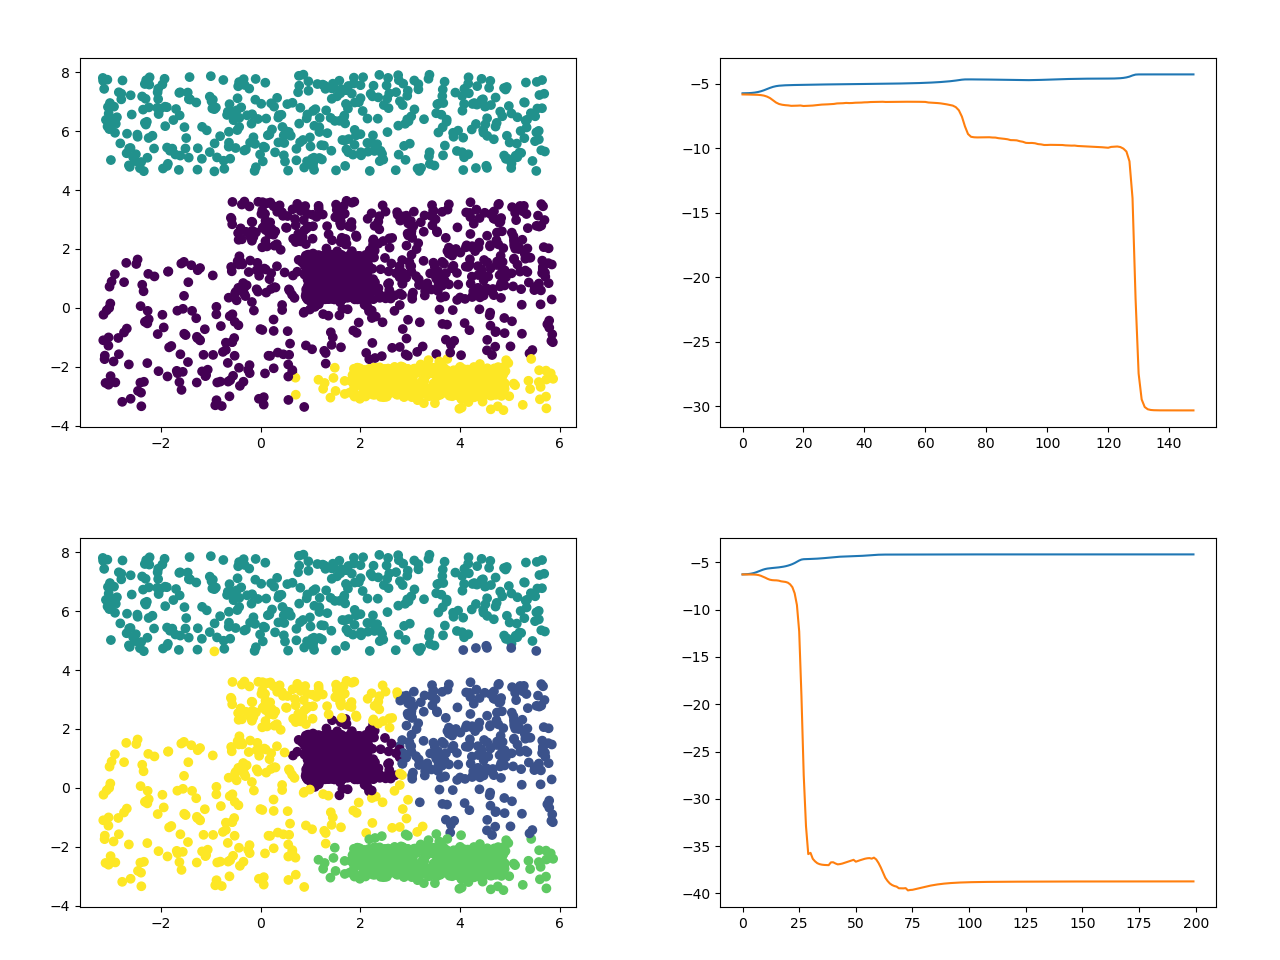
\includegraphics[width=120mm]{figs/gmm_ds5_orthog_plt_ll.png}
	\caption{Results for the sixth data set. TL: clustering with $k = 3$, TR: log likelihood with $k = 3$, BL: clustering with $k = 5$, BR: log likelihood with $k = 5$.}
\end{figure}

~\\
~\\
~\\
~\\
~\\
~\\
~\\
~\\
~\\
~\\
~\\
~\\
~\\
~\\
~\\
~\\
~\\
~\\
~\\
~\\
~\\
~\\
~\\
~\\
~\\
~\\
~\\
~\\
~\\

\section{Q2}

Using full covariance matrices does alleviate some of the problems outlined 
above. This is best illustrated with the first data set. Now, the clusters are 
angled to fit the data set better. (See figure 11.)

\begin{figure}[!ht]
	\centering
	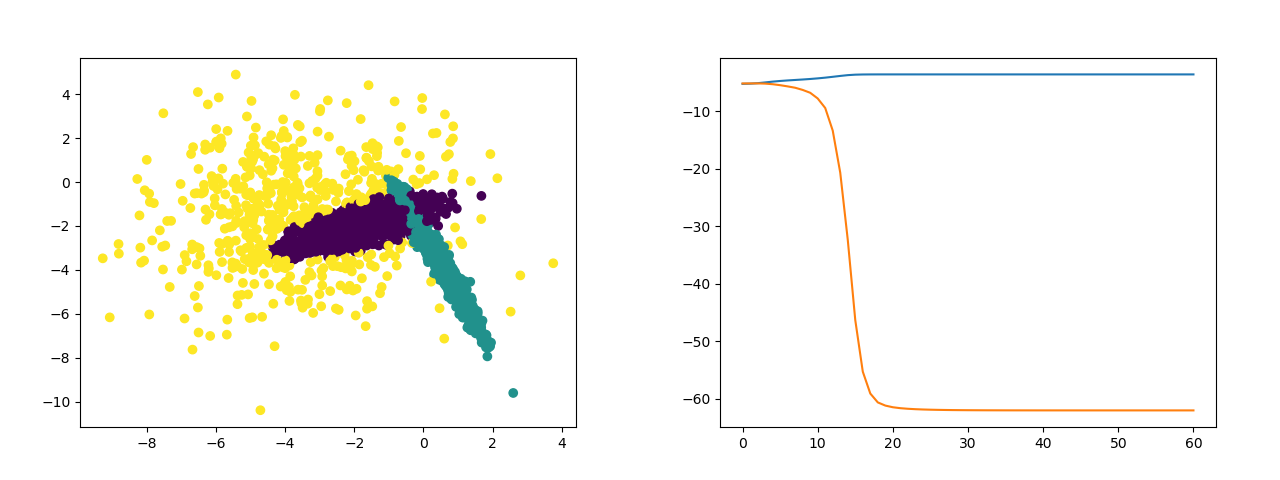
\includegraphics[width=120mm]{figs/gmm_ds0_k3_covar_plt_ll.png}
	\caption{With a full covariance matrix, the angles of the clusters of the 
        original data set are much better preserved.}
\end{figure}

In addition, the log likelihood plot looks typical, similar to those above. The 
algorithm is able to stop early, after only 60 iterations, because the GMM has 
converged to a local extremum.

However, even with the full covariance matrix, some data sets remain difficult 
to cluster. Consider the fifth data set. (See figure 12.)

\begin{figure}[!ht]
	\centering
	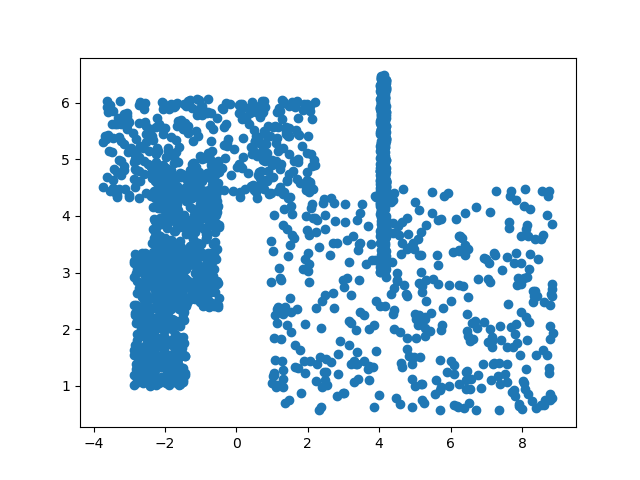
\includegraphics[width=60mm]{figs/gmm_ds4_kn_input.png}
	\caption{The fifth data set}
\end{figure}

Here, it appears to me that there are five clusters, and the clusters are fairly 
easy to identify, as they are essentially the five rectangles (top-left, 
mid-left, bottom-left, bottom-right, and top-mid). However, the key insight here 
is that these clusters are not Gaussian. The samples look to be taken from each 
point within the respective rectangles with an equal probability. To approach 
such a probability distribution, the peak of the best-fit Gaussian would need to 
be extremely wide, essentially wide enough to cover the entire rectangle. It 
simply doesn't work well, in this case. (See figure 13.)

\begin{figure}[!ht]
	\centering
	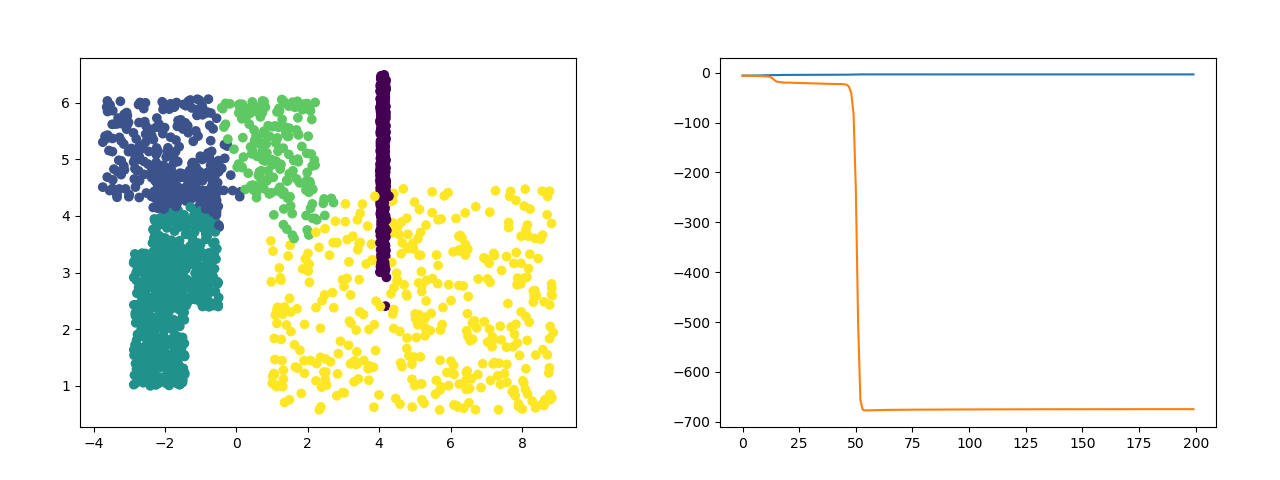
\includegraphics[width=120mm]{figs/gmm_ds4_k5_covar_plt_ll.png}
	\caption{Gaussian mixture models still have problems clustering 
        non-Gaussian data.}
\end{figure}

~\\
~\\
~\\
~\\
~\\
~\\
~\\
~\\
~\\
~\\
~\\

Not only is the clustering unsatisfactory, the log likelihood plot illustrates 
the unsatisfactory nature of the clustering. The test likelihood gets so bad 
that it essentially squishes the training likelihood into the top sliver of the 
plot. A test log likelihood that is that low is surely a sign that the 
clustering is not adequate.

One other phenomenon that is difficult to explain is the tiered nature of the 
log likelihood plot. Whereas most iterations only exhibited one period of 
rapid change in log likelihood, this plot has two: one at approximately 
iteration 12 and one at approximately iteration 50. I am not entirely sure what 
is causing that, but if we consider the curve for the objective function, 
abstractly, we may have reached a point where the objective function leveled 
out, but did not actually have a maximum at that point. This is best illustrated 
by the function $f(x) = x^3$. Here, at $x = 0$, the plot tapers out, but does 
not have an extremum. Something similar could be happening with the log 
likelihood, and thus the progression of the algorithm is hampered.

\section{Conclusion}

Though Gaussian mixture models are a very powerful clustering tool, they have 
some limitations. First, we must pick $k$. As illustrated by the log likelihood 
charts above, if we choose a bad $k$, our test log likelihood will be much lower 
than if we had chosen a good $k$. In two dimensions, it is fairly easy to 
visualize the data to determine what $k$ should be, but, for higher dimensions, 
picking $k$ becomes another task altogther. Some methods exist to alleviate this 
problem, like calculating the silhouette score and picking $k$ close to $log(N)$, 
but it will always be a parameter that needs to be tuned.

Second, Gaussian mixture models require a random initialization. For good values 
of $k$ with Gaussian data, different trials often converge to the same clustering. 
However, if the data is not Gaussian or we have picked a bad $k$, different 
trials will result in different clustering. Oftentimes, even after running 
several trials, it is still hard to determine which of these different 
clusterings should be used.

In addition, Gaussian mixture models cannot accurately cluster data that is not 
Gaussian, as we saw in the fifth data set.

Finally, to save computation, 
diagonal covariance matrices can be used, but they should only be used with 
data whose features are independent.

\end{document}